\label{ch:designs}

In addition to the MapReduce style data-analytics, there is a set of data analysis workflows that do not necessarily conform to the MapReduce abstraction.
Their tasks can be heterogeneous, implementing a diverse set of functionalities that are compute-intensive.
As a consequence, data-parallel frameworks, like Spark and Dask may not be the most suitable choice for their execution.
%Furthermore, the volume and scale of data justifies the use to parallelism and High Performance Computing (HPC) resources.
From a middleware perspective, the design and architectural space is large and the lack of performance analysis makes it difficult to select among equivalent implementations.

From a design perspective, a promising approach is isolating tasks from execution management.
Tasks are assumed to be self-contained programs which are executed in the operating system (OS) environment of HPC compute nodes.
Compared to approaches in which tasks are functions or methods, a program-based approach offers several benefits as, for example, simplified implementation of execution management, support of general purpose programming models, and separate programming of management and domain-specific functionalities.
Nonetheless, program-based designs also impose performance limitations, including OS-mediated intertask communication and task spawning overheads, as programs execute as OS processes and do not share a memory space.

Due to their performance limitations, program-based designs of computing frameworks are best suited to execute compute-intense workflows in which each task requires a certain amount of parallelism and runs from several minutes to hours.
The emergence of workflows that require heterogeneous, compute-intense tasks to process large amount of data is pushing the boundaries of program-based designs, especially when scale requirements suggest the use of modern HPC infrastructures with large number of CPUs/GPUs and dedicated data facilities.

We use a paradigmatic use case workflow from the polar science domain to evaluate three alternative task-based designs, and experimentally characterize and compare their performance.
Our use case requires us to analyze satellite images of Antarctica to detect pack-ice seals taken across a whole calendar year.
The resulting dataset consists of $3,097$ images for a total of $\approx4$~TB.
The use case requires us to repeatedly process these images, running both CPUs and GPUs code that exchange several GB of data.
The first design uses a pipeline to independently process each image, while the second and third designs use the same pipeline to process a series of images with differences in how images are bound to available compute nodes.

The chapter is organized as follows.
Section~\ref{sec:ucase} presents the use case and discusses it computational requirements as well as its task-based workflow.
In \S~\ref{sec:design}, we discuss the three architecturally equivalent design to support task-based workflows.
 \S\ref{sec:des_experiments} presents a performance evaluation of the designs and discusses the lessons learned.

\section{Satellite Imagery Analysis Application}
\label{sec:ucase}
Imagery employed by ecologists as a tool to survey populations and ecosystems come from a wide range of sensors, e.g., camera-trap surveys~\cite{karanth1995estimating} and aerial imagery transects~\cite{western2009impact}.
Very High Resolution (VHR) satellite imagery provides an effective alternative to perform large scale surveys at locations with poor accessibility such as surveying Antarctic fauna~\cite{lynch2012detection}.
To take full advantage from increasingly large VHR imagery, and reach the spatial and temporal breadths required to answer ecological questions, it is paramount to automate image processing and labeling.

Convolutional Neural Networks (CNN) represent the state-of-the-art for nearly every computer vision routine.
For instance, ecologists have successfully employed CNNs to detect large mammals in airborne imagery~\cite{kellenberger2018detecting,polzounov2016right}, and camera-trap survey imagery~\cite{norouzzadeh2018automatically}.
We use a Convolutional Neural Network (CNN) to survey Antarctic pack-ice seals in VHR imagery.
Pack-ice seals are a main component of the Antarctic food web~\cite{fabra2008convention}: estimating the size and trends of their populations is key to understanding how the Southern Ocean ecosystem copes with climate change~\cite{hillebrand2018climate} and fisheries~\cite{reid2019climate}.

This use case workflow processes WorldView 3 (WV03) panchromatic imagery, which has the highest available resolution for commercial satellite imagery.
%We use the best performing CNN model~\cite{goncalves2020sealnet} on an archive of over $3,097$ WV03 images, with a total dataset size of $\approx4$~TB.
Due to limitations on GPU memory, it is necessary to tile WV03 images into smaller patches before sending input imagery through the seal detection CNN.
Taking tiled imagery as input, the CNN outputs the latitude and longitude of each detected seal.
%While the raw model output still requires statistical treatment, such `mock-run' emulates the scale necessary to perform a comprehensive pack-ice seal census.
We order the tiling and seal detection stages into a pipeline that can be run with different imagery datasets.
This allows domain scientists to create seal abundance time series that can aid in Southern Ocean monitoring.
To create this time series, domain scientists define a computational campaign where each workflow analyzes imagery from different calendar years or seasons.


\section{Workflow Design and Implementation}\label{sec:design}
Computationally, the use case described in~\S\ref{sec:ucase} presents three main challenges: heterogeneity, scale and repeatability.
The images of the use case dataset vary in size with a wide distribution.
Each image requires tiling, per tile counting of seal populations and result aggregation across tiles.
Tiling is memory intensive while counting is computationally intensive, requiring CPU and GPU implementations, respectively.

We address these challenges by codifying image analysis into a workflow.
We then execute this workflow on HPC resources, leveraging the concurrency, storage systems and compute speed they offer to reduce time to completion.
Typically, this type of workflow consists of a sequence (i.e., pipeline) of tasks, each performing part of the end-to-end analysis on one or more images.
The implementation of this workflow varies, depending on the API of the chosen workflow system and its supported runtime system.
Here, we compare two common designs: one in which each image is processed independently by a dedicated pipeline; the other in which a pipeline processes multiple images.

Note that both designs separate the functionalities required to process each image from the functionalities used to coordinate the processing of multiple images.
This is consistent with moving away from vertical, end-to-end single-point solutions, favoring designs and implementations that satisfy multiple use cases, possibly across diverse domains.
Accordingly, the two designs we consider, implement, and characterize use two tasks (i.e., programs) to implement the tiling and counting functionalities required by the use case.

Both designs are functionally equivalent, in that they both enable the analysis of the given dataset.
Nonetheless, each design leads to different amounts of concurrency, resource utilization and overheads, depending on data/compute affinity, scheduling algorithm, and coordination between CPU and GPU computations.
Based on a performance analysis, it will be possible to know which design entails the best tradeoffs for common metrics as total execution time or resource utilization.

Consistent with HPC resources currently available for research and our use case, we make three architectural assumptions: 
\begin{inparaenum}[(1)]
    \item each compute node has $c$ CPUs;
    \item each compute node has $g$ GPUs where $g \le c$; and
    \item each compute node has enough memory to enable concurrent execute of a certain number of tasks.
\end{inparaenum}
As a result, at any given point in time there are $C = n\times c$ CPUs and $G = n\times g$ GPUs available, where $n$ is the number of compute nodes.

\begin{figure}[H]
    \centering
    \begin{subfigure}[b]{0.75\textwidth}
        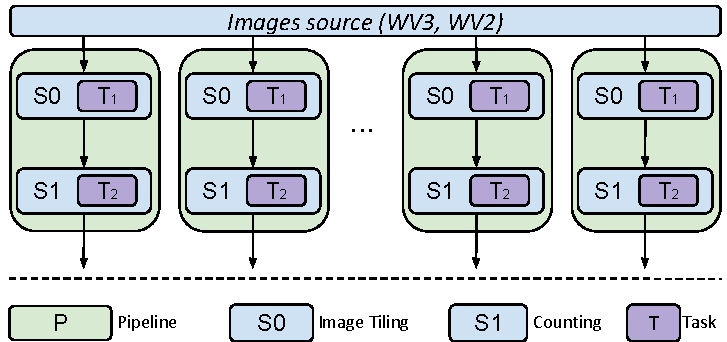
\includegraphics[width=\linewidth]{figures/designs/SealsDesign1.pdf}
        \caption{}
        \label{fig:seals_design1}
    \end{subfigure}\\
    ~ 
    \begin{subfigure}[b]{0.75\textwidth}
        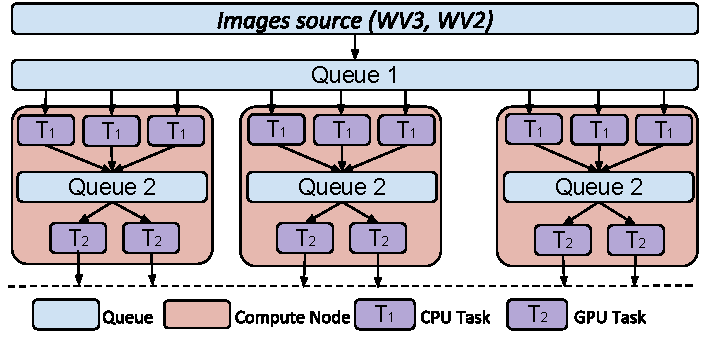
\includegraphics[width=\linewidth]{figures/designs/SealsDesign2.pdf}
        \caption{}\label{fig:seals_design2}
    \end{subfigure}\\
    ~ 
    \begin{subfigure}[b]{0.75\textwidth}
        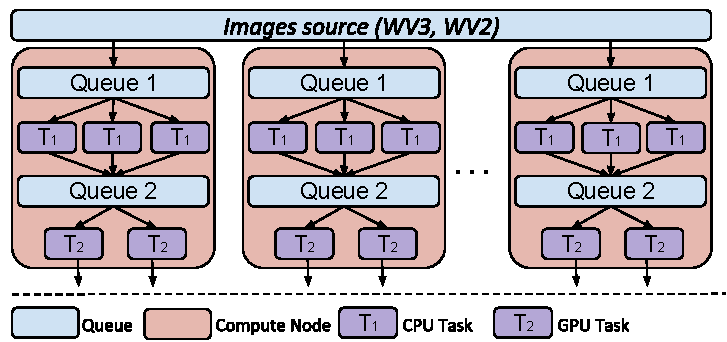
\includegraphics[width=\linewidth]{figures/designs/SealsDesign3.pdf}
        \caption{}\label{fig:seals_design3}
    \end{subfigure}
    \caption{Design approaches to implement the workflow required for the Seals use case.~\ref{fig:seals_design1}
        --\textbf{Design 1}: Pipeline, stage and task based design.~\ref{fig:seals_design2}
        --\textbf{Design 2}: Queue based design with a single queue for all the tiling tasks.~\ref{fig:seals_design3}
        --\textbf{Design 2.A}: Queue based design with multiple queues for the tiling tasks.}\label{fig:designs}
\end{figure}

% ---------------------------------------------------------------------------
\subsection{Design 1: One Image per Pipeline}
\label{ssec:approach1}\label{des1}


% ---------------------------------------------------------------------------
% Design
% ---------------------------------------------------------------------------

We specify the workflow for counting the number of seals in a set of images as a set of pipelines.
Each pipeline is composed of two stages, each with one type of task.
The task of the first stage gets an image as input and generates tiles of that image as output.
The task of the second stage gets the generated tiles as input, counts the number of seals found in each tile and outputs the aggregated result for the whole image.

Formally, we define two types of tasks:
\begin{itemize}
    \item $T_{1} = <I, f_{I}, t>$, where $I$ is an image, $f_{I}$ is a tiling function and $t$ is a set of tiles that correspond to $I$.
    \item $T_{2} = <t, f_{A}, S>$, where $f_{A}$ is a function that counts seals from a set of tiles and $S$ is the number of seals.
\end{itemize}


% ---------------------------------------------------------------------------
% Implementation
% ---------------------------------------------------------------------------
Tiling in $T_{1}$ is implemented with OpenCV~\cite{bradski2000opencv} and Rasterio~\cite{gillies2013rasterio} in Python.
Rasterio allows us to open and convert a GeoTIFF WV3 image to an array.
The array is then partitioned to sub\-arrays based on a user-specified scaling factor.
Each sub\-array is converted to an compressed image via OpenCV routines and saved to the filesystem.

Seal counting in $T_{2}$ is performed via a Convolutional Neural Network (CNN) implemented with PyTorch~\cite{paszke2017automatic}.
The CNN counts the number of seals for each tile of an input image.
When all tiles are processed, the coordinates of the tiles are converted to the geographical coordinates of the image and saved in a file, along with the number of counted seals.
Note that the number of seals in an tile does not affect the execution of the network, i.e. the same number of operations will be executed.

Both tiling and seal counting implementations are invariant between the designs we consider.
This is consistent with the designs being task-based, i.e., each task exclusively encapsulates the capabilities required to perform a specific operation over an image or tile.
Thus, tasks are independent from the capabilities required to coordinate their execution, whether each task processes a single image or sequence of images.

We implemented Design~1 via EnTK, a workflow engine which exposes an API based on pipelines, stages, and tasks~\cite{balasubramanian2018harnessing}.
The user can define a set of pipelines, where each pipeline has a sequence of stages, and each stage has a set of tasks.
Stages are executed respecting their order in the pipeline while the tasks in each stage can execute concurrently, depending on resource availability.

For our use case, EnTK has three main advantages compared to other workflow engines:
\begin{inparaenum}[(1)]
    \item it exposes pipelines and tasks as first-order abstractions implemented in Python;
    \item it is specifically designed for concurrent management of up to $10^5$ pipelines; and
    \item it supports RADICAL-Pilot.
\end{inparaenum} 
Together, these features address the challenges of heterogeneity, scale and repeatability: users can encode multiple pipelines, each with different types of tasks, executing them at scale on HPC machines without explicitly coding parallelism and resource management.

When implemented in EnTK, the use case workflow maps to a set of pipelines, each with two stages $St_{1}$, $St_{2}$.
Each stage has one task $T_{1}$ and $T_{2}$ respectively.
The pipeline is defined as $P = (St_{1},St_{2})$.
For our use case the workflow consists of $N$ pipelines, where $N$ is the number of images.

Figure~\ref{fig:seals_design1} shows the workflow.
For each pipeline, EnTK submits the task of stage $St_{1}$ to the runtime system (RTS).
As soon as the task finishes, the task of stage $St_{2}$ is submitted for execution.
This design allows concurrent execution of pipelines and, as a result, concurrent analysis of images, one by each pipeline.
Since pipelines execute independently and concurrently, there are instances where $St_{1}$ of a pipeline executes at the same time as $St_{2}$ of another pipeline.

Design~1 has the potential to increase utilization of available resources as each compute node of the target HPC machine has multiple CPUs and GPUs.
Importantly, computing concurrency comes with the price of multiple reading and writing to the filesystem on which the dataset is stored.
This can cause I/O bottlenecks, especially if each task of each pipeline reads from and writes to the same filesystem, possibly over a network connection.

We used a tagged scheduler for EnTK's RTS to avoid I~/O bottlenecks.
This scheduler schedules $T_{1}$ of each pipeline on the first available compute node, and guarantees that the respective $T_{2}$ is scheduled on the same compute node.
As a result, compute/data affinity is guaranteed among co-located $T_{1}$ and $T_{2}$.
While this design avoids I~/O bottlenecks, it may reduce concurrency when the performance of the compute nodes and/or the tasks is heterogeneous: $T_{2}$ may have to wait to execute on a specific compute node while another node is free.


% ---------------------------------------------------------------------------
\subsection{Design 2: Multiple images per pipeline}\label{ssec:approach2}

Design~2 implements a queue-based design.
We introduce two tasks $T_{1}$ and $T_{2}$ as defined in~\S\ref{ssec:approach1}.
Contrary to Design 1, these tasks are started and then executed for as long as data and resources are available, processing input images at the rate taken to process each image.
The number of concurrent $T_{1}$ and $T_{2}$ depends on available resources, including CPUs, GPUs, and RAM.

For implementing Design~2, we do not need EnTK, as we submit a bag of $T_{1}$ and $T_{2}$ tasks via the RADICAL~-Pilot RTS, and manage the data movement between tasks via queues.
As shown in Fig.~\ref{fig:seals_design2}, Design 2 uses one queue (Queue 1) for the dataset, and another queue (Queue 2) for each compute node.
For each compute node, each $T_{1}$ pulls an image from Queue 1, tiles that image and then queues the resulting tiles to Queue 2.
The first available $T_{2}$ on that compute node, pulls those tiles from Queue 2, and counts the seals.

%To communicate data and control signals between queues and tasks, we defined a communication protocol with three entities: Sender, Receiver, and Queue. 
%Sender connects to Queue and pushes data.
%When done, Sender informs Queue and disconnects.
%Receiver connects to Queue and pulls data.
%If there are no data in Queue but Sender is connected, Receiver pulls a ``wait'' message, waits, and pulls again after a second.
%When there are no data in Queue or Sender is not connected to Queue, Receiver pulls an ``empty'' message, upon which it disconnects and terminates.
%This ensures that tasks are executing, even if starving, and that all tasks are gracefully terminating when all images are processed.

Note that Design~2 load balances $T_{1}$ tasks across compute nodes but  balances $T_{2}$ tasks only within each node.
For example, suppose that $T_{1}$ on compute node $A$ runs two times faster than $T_{1}$ on compute node $B$.
Since both tasks are pulling images from the same queue, $T_{1}$ of $A$ will process twice as many images as $T_{1}$ of $B$.
Both $T_{1}$ of $A$ and $B$ will execute for around the same amount of time until Queue 1 is empty, but Queue 2 of $A$ will be twice as large as Queue 2 of $B$.
$T_{2}$ tasks executing on $B$ will process half as many images as $T_{2}$ tasks on $A$, possibly running for a shorter period of time, depending on the time taken to process each image.

In principle, Design~2 can be modified to load balance also across Queue 2 but in practice, as discussed in~\S\ref{ssec:approach1}, this would produce I/O bottlenecks.
Load balancing across $T_{2}$ tasks would require for all tiles produced by $T_{1}$ tasks to be written to and read  from a  shared filesystem.
Keeping Queue 2 local to each compute node enables using the filesystem local to each compute node.

% ---------------------------------------------------------------------------
\subsubsection{Design 2.A: Uniform image dataset per pipeline}
\label{sssec:approach2a}

The lack of load balancing of $T_{2}$ tasks in Design 2 can be mitigated by introducing a queue in each node from where $T_{1}$ tasks pull images.
This allows early binding of images to compute nodes, i.e., deciding the distribution of images per node before executing $T_{1}$ and $T_{2}$.
As a result, the execution can be load balanced among all available nodes, depending on the correlation between image properties and image execution time.

Figure~\ref{fig:seals_design3} shows variation 2.A of Design~2.
The early binding of images to compute nodes introduces an overhead compared to using late binding via a single queue as in Design 2.
Nonetheless, depending on the strength of the correlation between image properties and execution time, design 2.A offers the opportunity to improve resource utilization.
While in Design 2 some node may end up waiting for another node to process a much larger Queue 2, in design 2.A this is avoided by guaranteeing that each compute node has an analogous payload to process.

\section{Experiments: Task Execution Time, Resource Utilization and Overheads}\label{sec:des_experiments}
%See if comparing performance is better.
We executed three experiments using GPU compute nodes of the XSEDE Bridges supercomputer.
These nodes offer 32 cores, 128 GB of RAM and two P100 Tesla GPUs.
We stored the dataset of the experiments and the output files on XSEDE Pylon5 Lustre filesystem.
We stored the tiles produced by the tiling tasks on the local filesystem of the compute nodes.
This way, we avoided creating a performance bottleneck by performing millions of reads and writes of $\approx700$~KB on Pylon5.
We submitted jobs requesting 4 compute nodes to keep the average queue time within a couple of days.
Requesting more nodes produced queue times in excess of a week.
In addition, we had full control over the nodes during execution and were not shared with other users.

The experiments dataset consists of $3,097$ images, ranging from $50$ to $2,770$~MB for a total of $\approx4$~TB of data.
The images size follows a normal distribution with a mean value of $1,304.85$~MB and standard deviation of $512.68$~MB.

For Design~1, 2 and 2.A described in~\S\ref{sec:design}, Experiment~1 models the execution time of the two tasks of our use case as a function of the image size (the only property of the images for which we found a correlation with execution time); Experiment~2 measures the total resource utilization of each design; and Experiment~3 characterizes the overheads of the middleware implementing each design.
Together, these experiments enable performance comparison across designs, allowing us to draw conclusions about the performance of heterogeneous task-based execution of data-driven workflows on HPC resources.

% ---------------------------------------------------------------------------
\subsection{Experiment~1: Design~1 Tasks Execution Time}
\label{ssec:des1analysis}

Fig.~\ref{fig:stage_0_execution} shows the execution time of the tiling task---defined as $T_{1}$ in~\S\ref{des1}---as a function of the image size.
We partition the set of images based on image size, obtaining 22 bins with a range of $125$~MB each starting from $50$~MB up to $2,800$~MB.
The average time taken to tile an image in each bin tends to increase with the size of the image.
The box-plots show some positive skew of the data with a number of data points  falling outside the assumed normal distribution.
There are also large standard deviations ($STD$, blue line) in most of the bins.
Thus, there is a weak correlation between task execution time and image size with a large spread  across all the image sizes.

\begin{figure}[t]
    \centering
    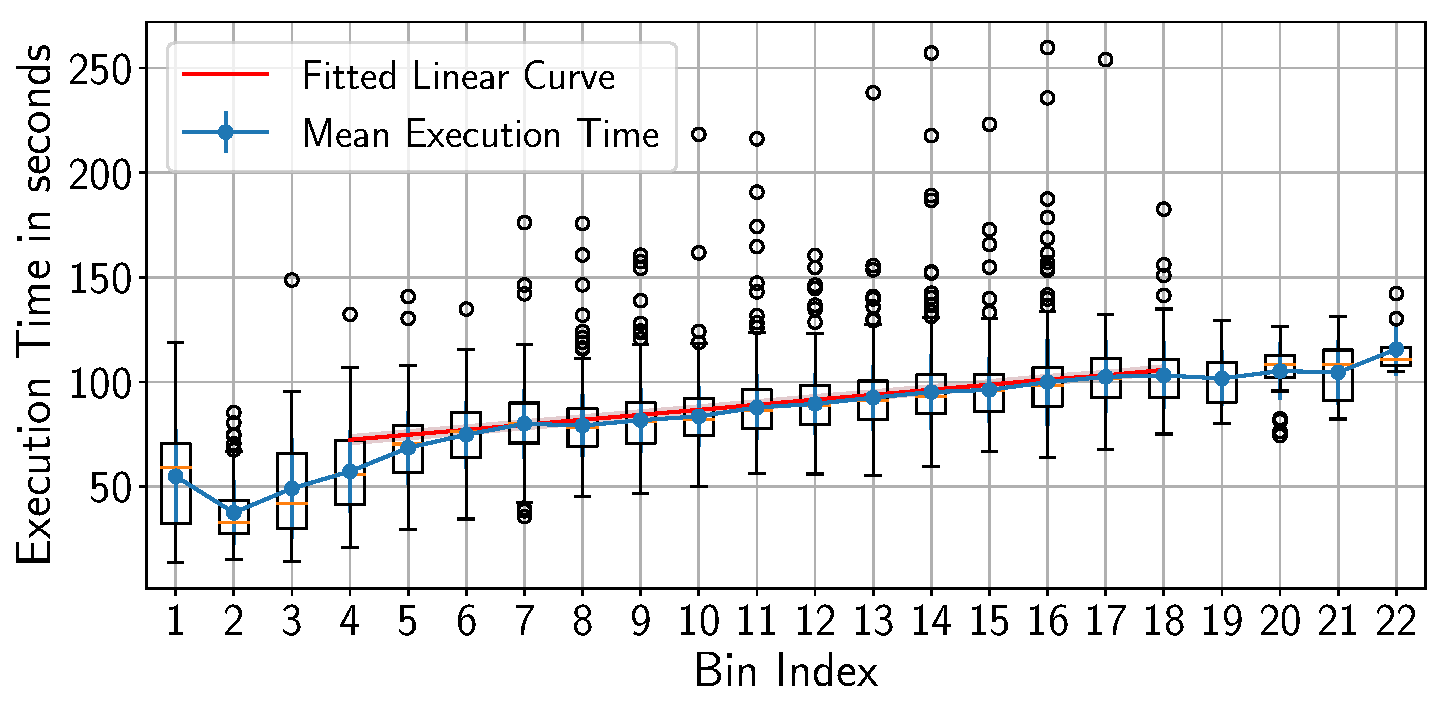
\includegraphics[width=0.75\textwidth]{figures/designs/stage_0_tx_box.pdf}
    \caption{Experiment~1, Design~1: Box-plots of $T_{1}$ execution time, mean and $STD$ for $125$~MB image size bins.
        Red line shows fitted linear function.}\label{fig:stage_0_execution}
\end{figure}

We explored the causes of the observed $STD$ by measuring how it varies in relation to the number of tiling tasks concurrently executing on the same node.
Fig.~\ref{fig:concurrency_test} shows the standard deviation of each bin of Fig.~\ref{fig:stage_0_execution}, based on the amount of used task concurrency.
We observe that $STD$ drops with increased concurrency but remains relatively stable between bins $\#6$ and $\#20$.
We attribute the initial dropping to how Lustre's caching improves the performance of an increasing number of concurrent requests.
Further, we observe that as the type of task and the compute node are the same across all our measures, the relatively stable and consistent $STD$ observed across degrees of task concurrency depends on fluctuations in the node performance.

\begin{figure}[t]
    \centering
    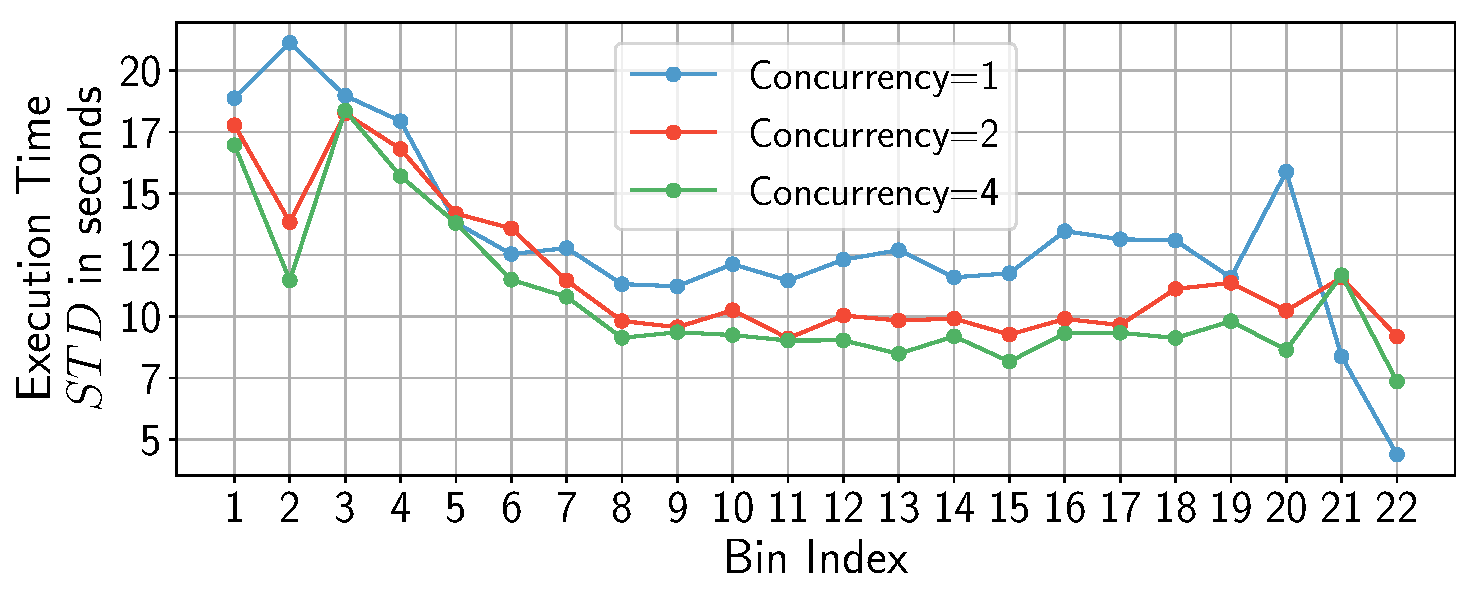
\includegraphics[width=.75\textwidth]{figures/designs/concerrency_std.pdf}
    \caption{$STD$ of $T_{1}$ execution time based on image size bin and number of concurrent tasks.
        Mostly dependent on compute node's performance and invariant across values of task concurrency.}\label{fig:concurrency_test}
\end{figure}

Fig.~\ref{fig:stage_0_execution} indicates that the execution time is a linear function of the image size between bin \#4 and bin \#18.
Bins $1-3$ and $19-23$ are not representative as the head and tail of the image sizes distribution contain less than $5\%$ of the image dataset.
We model the execution time as:
\begin{equation}
T(x) = \alpha \times x+\beta
\label{eq:des1_til}
\end{equation} where $x$ is the image size.


\begin{table*}[t]
    \scriptsize
    \centering
    \begin{tabular}{@{}cclrcl@{}}
        \toprule
        \textbf{Design}                                &
        \textbf{Fitted Data}                           &
        \textbf{$\alpha$ value}                        &
        \textbf{$\beta$ value}                         &
        \textbf{$R^2$ value}                           &
        \textbf{Figure}                                \\
        \midrule
        1                                              & 
        $T_{1}$                                  & 
        $1.92\times 10^{-2}$                           & 
        $60.49$                                        & 
        $0.97$                                         & 
        Fig.~\ref{fig:stage_0_execution}, red line     \\
        %
        1                                              & 
        $T_{2}$                                        & 
        $5.21\times 10^{-2}$                           & 
        $128.53$                                       & 
        $0.96$                                         & 
        Fig.~\ref{fig:stage_1_execution}, green line   \\
        %
        2                                              &
        $T_{1}$                                        &
        $3.17\times 10^{-2}$                           &
        $64.81$                                        &
        $0.92$                                         &
        Fig.~\ref{fig:stage_1_execution_des2}, red line     \\
		%
        2                                              &
        $T_{2}$                                        &
        $4.71\times 10^{-2}$                           &
        $95.83$                                        &
        $0.95$                                         &
        Fig.~\ref{fig:stage_2_execution_des2}, green line   \\
        2.A                                            &
        $T_{1}$                                        &
        $2.74\times 10^{-2}$                           &
        $49.03$                                        &
        $0.94$                                         &
        N/A     \\
		%
        2.A                                            &
        $T_{2}$.                                        &
        $4.80\times 10^{-2}$                           &
        $87.60$                                        &
        $0.95$                                         &
        N/A   \\
		\bottomrule
    \end{tabular}
    \caption{Fitted parameter values of Eq.~\ref{eq:des1_til} using a
             non-linear least squares algorithm to fit our experimental
             data.}\label{tab:fit_par_val}
\end{table*}

We found the parameter values of Eq.~\ref{eq:des1_til} by using a non-linear least squares algorithm to fit our experimental data, which are $\alpha= 1.92 \times 10^{-2}$, and $\beta = 60.49$ (see red line in Fig.~\ref{fig:stage_0_execution}).
$R^{2}$ of our fitting is $0.97$, showing a very good fit of the curve to the actual data.

The Standard Error of the estimation, $S_{error}$, reflects the precision of our regression.
The $S_{error}$ is equal to $1.93$, shown as the red shadow in Fig.~\ref{fig:stage_0_execution}.
From $R^{2}$ and $S_{error}$ we conclude that our estimated function is validated and is a good fit for the execution time of $T_{1}$ for Design~1.

% ---------------------------------------------------------------------------
% \subsubsection{\texorpdfstring{$St_2$}{St2} Stage Analysis}

Fig.~\ref{fig:stage_1_execution} shows the execution time of the seals counting task as a function of the image size.
Defined as $T_{2}$ in~\S\ref{des1}, this task presents a different behavior than $T_{1}$, as the code executed is different.
Note the slightly stronger positive skew of the data compared to that of Fig.~\ref{fig:stage_0_execution} but still consistent with our conclusion that deviations are mostly due to fluctuations in the compute node performance (i.e., different code but similar fluctuations).

\begin{figure}[t]
    \centering
    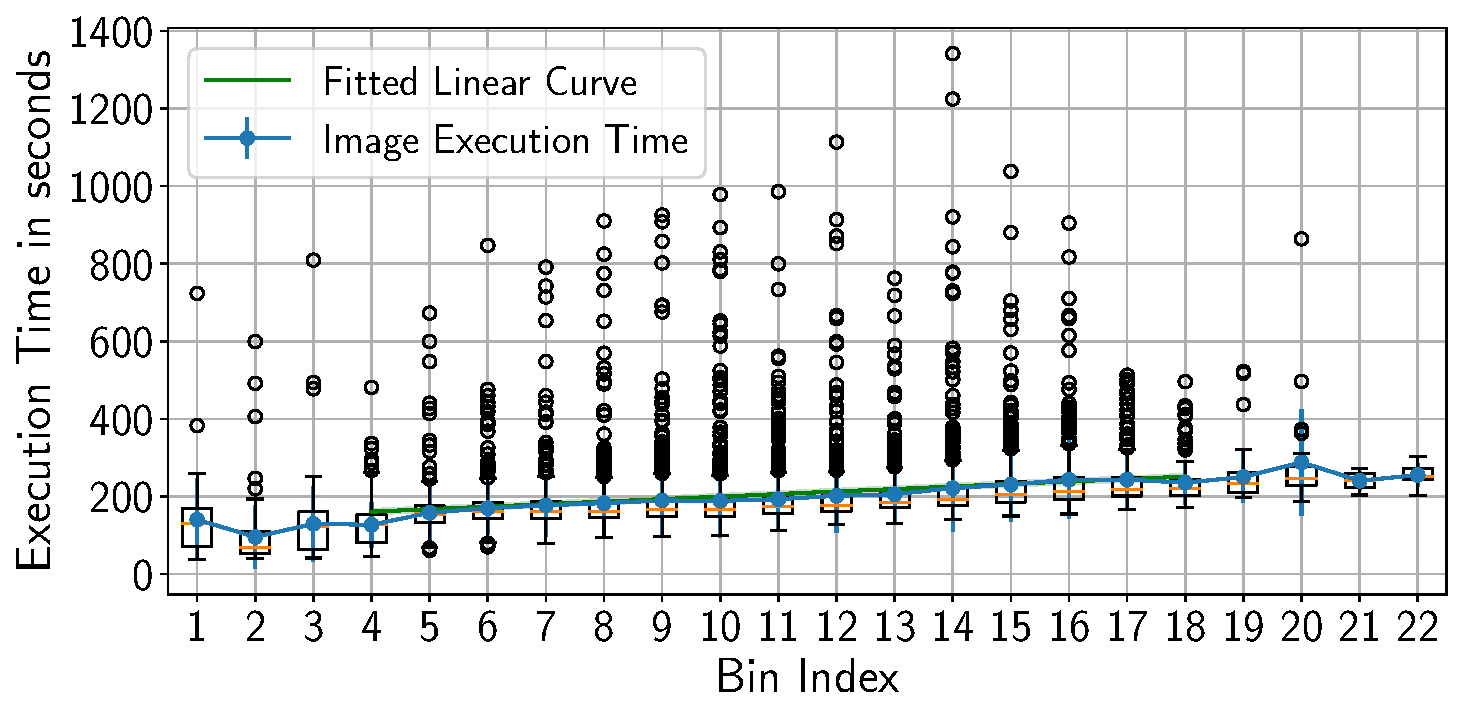
\includegraphics[width=0.75\textwidth]{figures/designs/stage_1_tx_box.pdf}
    \caption{Experiment~1, Design~1: Box-plots of $T_{2}$ execution time, mean and $STD$ for $125$~MB image size bins.
        Green line shows fitted linear function.}
    \label{fig:stage_1_execution}
\end{figure}

Similar to $T_{1}$, Fig.~\ref{fig:stage_1_execution} shows a weak correlation between the execution time of $T_{2}$ and image size.
In addition, the variance per bin is relatively similar across bins, as expected based on the analysis of $T_{1}$.
The box-plot and the mean execution time indicate that a linear function is a good candidate for a model of $T_{2}$.
As in Eq.~\ref{eq:des1_til}, we fitted a linear function to the execution time as a function of the image size for the same bins as $T_{1}$.

Using the same method we used with $T_{1}$, we produced the green line in Fig.~\ref{fig:stage_1_execution} with parameter values $\alpha = 5.21 \times 10^{-2}$ and $\beta = 128.53$.
$R^{2}$ is $0.96$, showing a good fit of the line to the actual data, while $S_{error}$ is $5.73$, slightly higher than for $T_{1}$.
As a result, we conclude that our estimated function is validated and is a good fit for the execution time of $T_{2}$ for Design~1.

% ---------------------------------------------------------------------------
\subsection{Experiment~1: Design~2 Tasks Execution Time}

Fig.~\ref{fig:stage_1_execution_des2} shows the execution time of $T_{1}$ as a function of the image size for Design~2.
In principle, design differences in middleware that execute tasks as independent programs should not directly affect task execution time.
In this type of middleware, task code is independent from that of the middleware: once tasks execute, the middleware waits for each task to return.
Nonetheless, in real scenarios with concurrency and heterogeneous tasks, the middleware may perform operations on multiple tasks while waiting for others to return.
Accordingly, in Design~2 we observe an execution time variation comparable to that observed with Design~1 but Fig.~\ref{fig:stage_1_execution_des2} shows a stronger positive skew of the data in Design~2 than Fig.~\ref{fig:stage_0_execution} in Design~1.

\begin{figure}[t]
    \centering
    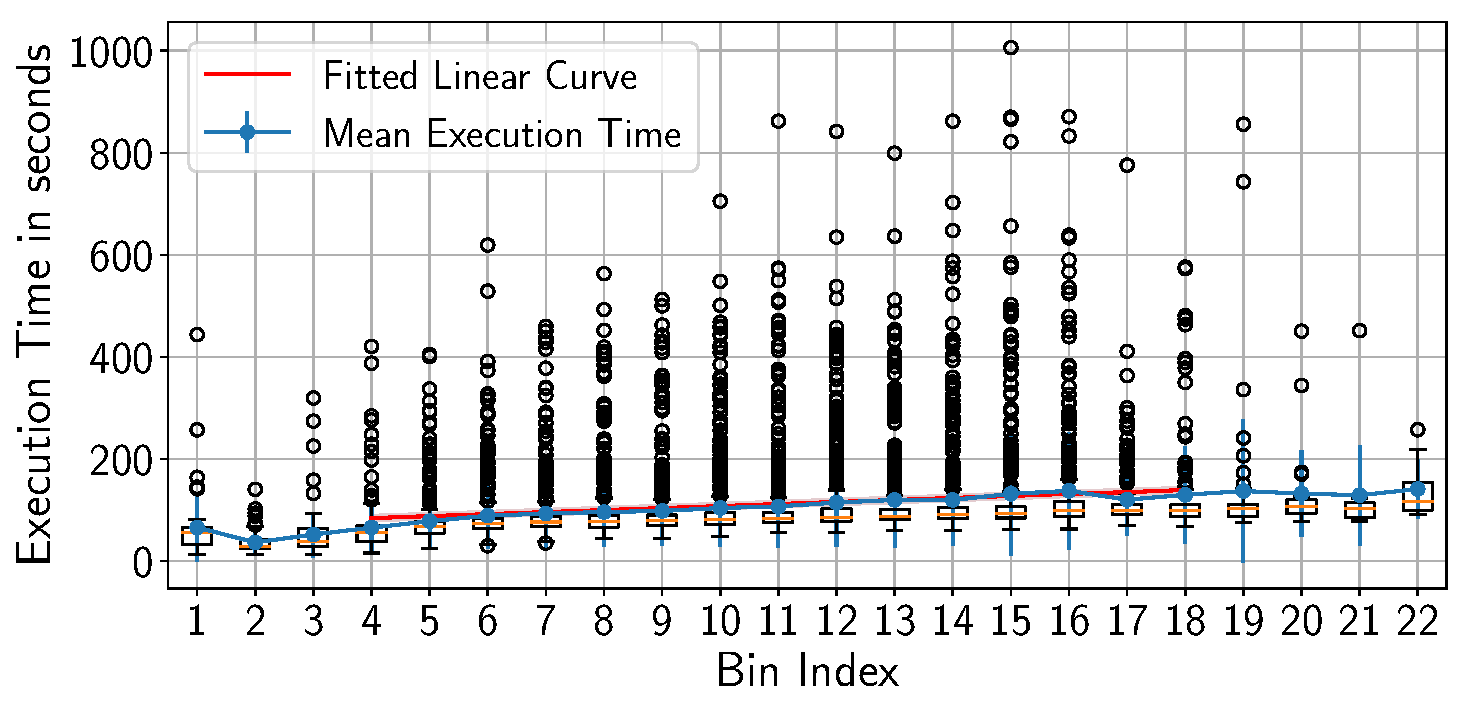
\includegraphics[width=0.75\textwidth]{figures/designs/stage_0_tx_box_des2.pdf}
    \caption{Experiment~1, Design~2: Box-plots of $T_{1}$ execution time, mean and $STD$ for $125$~MB image size bins.
        Red line shows fitted linear function.}\label{fig:stage_1_execution_des2}
\end{figure}


We investigated the positive skew of the data observed in Fig.~\ref{fig:stage_1_execution_des2} by comparing the system load of a compute node when executing the same number of tiling tasks in Design~1 and 2.
The system load of Design~2 was higher than that of Design~1.
Compute nodes have the same hardware and operating system, and run the same type and number of system programs.
As we used the same type of task, image and task concurrency, we conclude that the middleware implementing Design~2 uses more compute resources than that used for Design~1.
Due to concurrency, the middleware of Design~2 competes for resources with the tasks, momentarily slowing down their execution.
This is consistent with the architectural differences across the two designs: Design~2 requires resources to manage queues and data movement while Design~1 has only to schedule and launch tasks on each node.

We fitted Eq.~\ref{eq:des1_til} to the execution time of $T_1$ for Design~2, obtaining $\alpha = 3.174 \times 10^{-2}$ and $\beta = 64.81$.
The fitting produced the red line in Fig.~\ref{fig:stage_1_execution_des2}.
$R^{2}$ is $0.92$, showing a good fit of the curve to the data and $S_{error}$ is $5.50$, validating our estimated function.
$R^2$ and especially $S_{error}$ are worse compared to Design~1, an expected difference based on the positive skew of the data observed in Design~2.

% ------------
% \subsubsection{\texorpdfstring{$St_2$}{St2} Stage Analysis}

Fig.~\ref{fig:stage_2_execution_des2} shows that Design~2 also produces a much stronger positive skew of $T_{2}$ execution time compared to executing $T_{2}$ with Design~1.
$T_{2}$ executes on GPU and $T_{1}$ on CPU but their execution times produce comparable skew in Design~2.
This further supports our hypothesis that the long tail of the distribution of $T_{1}$ and especially $T_{2}$ execution times depends on the competition for main memory and I/O between the middleware implementing Design~2 and the executing tasks.


\begin{figure}[t]
    \centering
    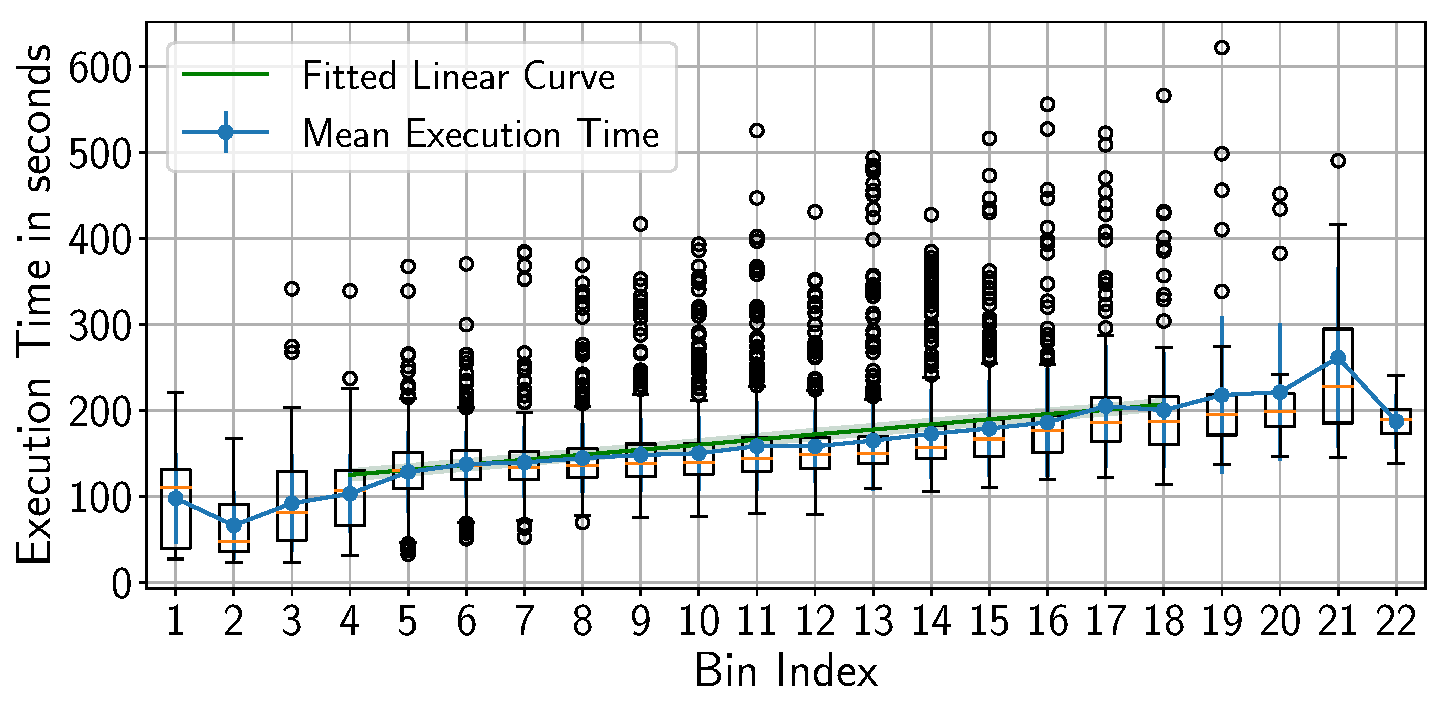
\includegraphics[width=0.75\textwidth]{figures/designs/stage_1_tx_box_des2.pdf}
    \caption{Experiment~1, Design~2: Box-plots of $T_{2}$ execution time, mean and $STD$ for $125$~MB image size bins.
        Green line shows fitted linear function.}\label{fig:stage_2_execution_des2}
\end{figure}

Fitting the model gives $\alpha = 4.71 \times 10^{-2}$ and $\beta = 95.83$.
$R^{2}$ is $0.95$ and $S_{error}$ of $5.96$.
As a result, the model is validated and a good candidate for the experimental data.
We attribute the difference between these values and those of the model of $T_{2}$ for Design~1 to the already described positive skew of execution times in Design~2.

% ------------
\subsubsection{Design~2.A} Similarly to the analysis in Design~1 and 2 we fitted data from Design~2.A to Eq.~\ref{eq:des1_til}.
For $T_{1}$ the fit gives $\alpha=2.74\times10^{-2}$ and $\beta=49.03$, with $R^{2}$ and $S_{error}$ of $0.94$ and $3.89$ respectively.
For $T_{2}$ the fit gives $\alpha=4.8\times10^{-2}$ and $\beta=87.36$, with $R^{2}=0.95$ and $S_{error}=6.19$.
Both models are therefore a good fit for the data and are validated.

The results of our experiments indicate that, on average and across multiple runs, there is a decrease in the execution time of $T_{1}$ and an increase in that of $T_{2}$ compared to Design~2.
Design~2.A requires one queue more than Design~2 for $T_{1}$ and therefore more resources for Design~2.A implementation.
This can explain the slowing of $T_{2}$ but not the speedup of $T_{1}$.
This requires further investigation, measuring whether the performance fluctuations of compute nodes are larger than measured so far.

As discussed in~\S\ref{ssec:approach2}, balancing of workflow execution differs between Design~2 and Design~2.A. Fig.~\ref{fig:design2_timeline} shows that each $T_{1}$ task can work on a different number of images but all $T_{1}$ tasks concurrently execute for a similar duration.
The four distributions in Fig.~\ref{fig:design2_timeline} also show that this balancing can result in different input distributions for each compute node, affecting the total execution time of $T_{2}$ tasks on each node.
Thus, Design~2 can create imbalances in the time to completion of $T_{2}$, as shown by the red bars in Fig.~\ref{fig:design2_timeline}.

\begin{figure}[t]
    \centering
    \begin{subfigure}[b]{0.75\textwidth}
        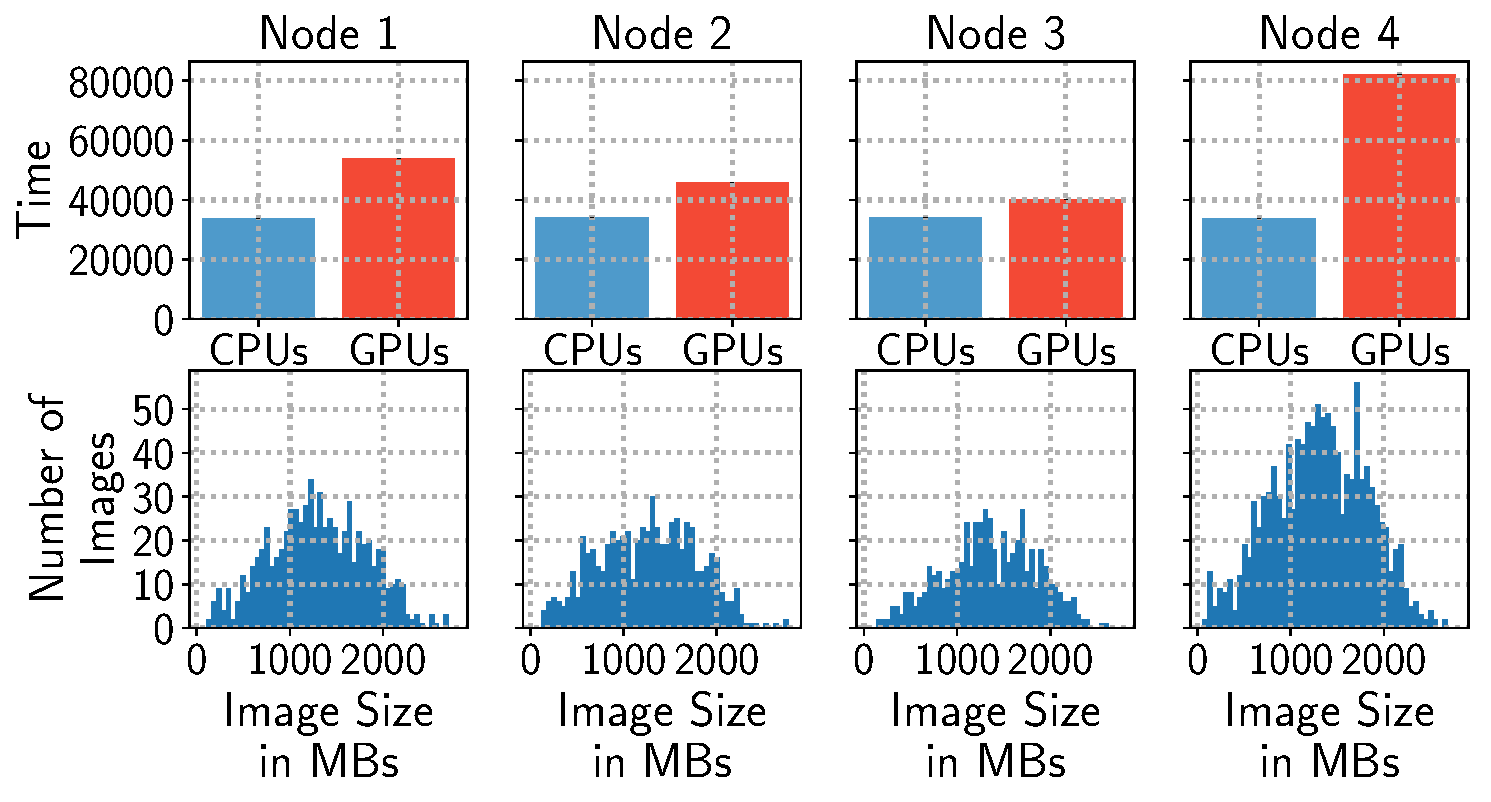
\includegraphics[width=\linewidth]{figures/designs/design2_timelines.pdf}
        \caption{}
        \label{fig:design2_timeline}
    \end{subfigure}\\
    ~ 
    \begin{subfigure}[b]{0.75\textwidth}
        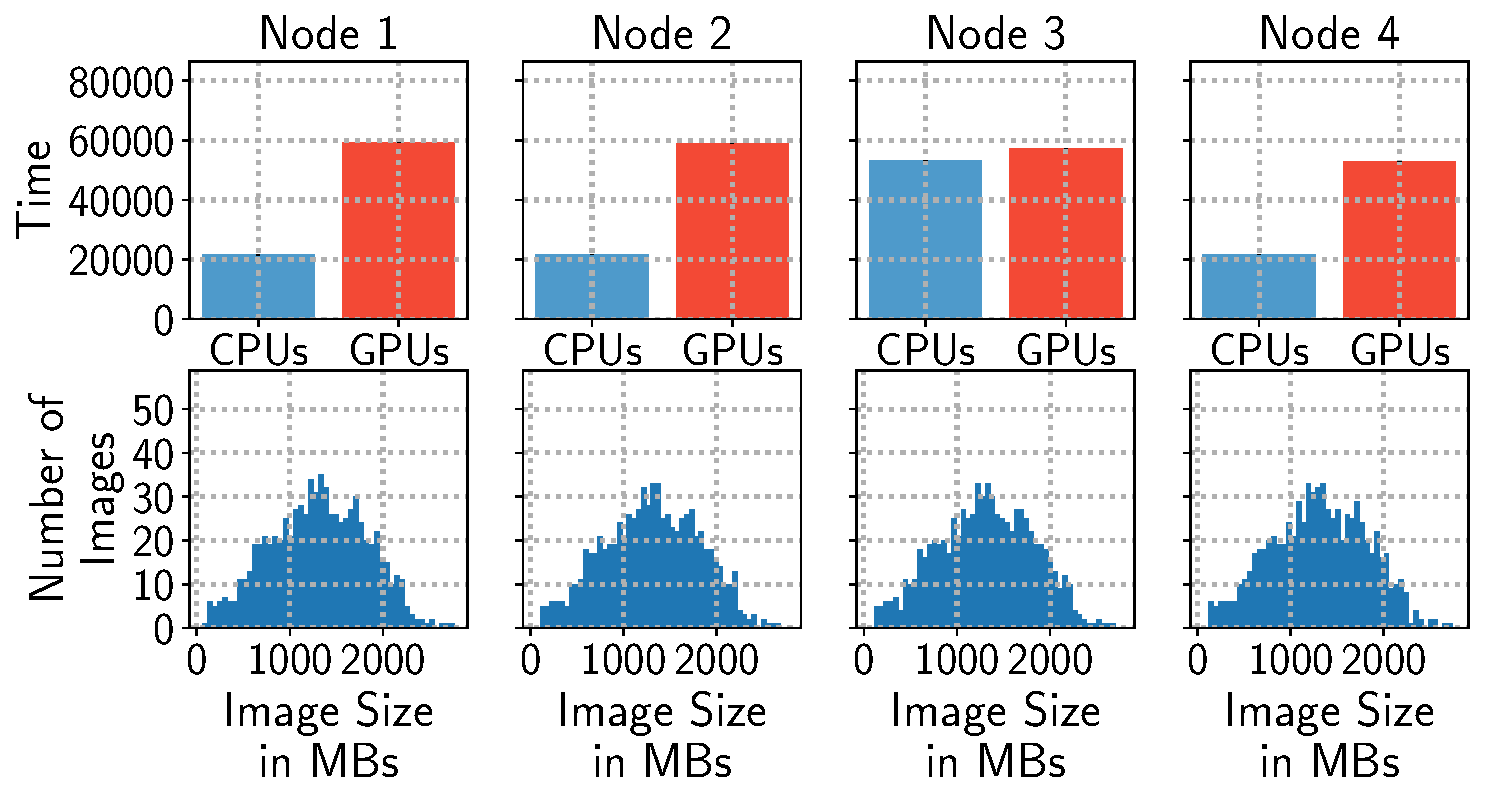
\includegraphics[width=\linewidth]{figures/designs/design2a_timelines.pdf}
        \caption{}
        \label{fig:design2a_timeline}
    \end{subfigure}
    \caption{Execution time of $T_{1}$ (blue) and $T_{2}$ (red),
        and distributions of image size per node for (a) Design~2 and (b)
        Design~2.A.}
    \label{fig:design_balancing}
\end{figure}


Design~2.A addresses these imbalances by early binding images to compute nodes.
Comparing the lower part of Fig.~\ref{fig:design2_timeline} and Fig.~\ref{fig:design2a_timeline} shows the difference between the distributions of image size for each node between Design~2 and 2.A.
In Design~2.A, due to the modeled correlation between time to completion and the size of the processed image, the similar distribution of the size of the images bound to each compute node balances the total processing time of the workflow across multiple nodes.

Note that Fig.~\ref{fig:design_balancing} shows just one of the runs we perform for this experiment.
Due to the random pulling of images from a global queue performed by Design~2, each run shows different distributions of image sizes across nodes, leading to large variations in the total execution time of the workflow.
Fig.~\ref{fig:design2a_timeline} shows also an abnormal behavior of one compute node: For images larger than $1.5$GBs, Node 3 CPU performance is markedly slower than other nodes when executing $T_{1}$.
Different from Design~2, Design~2.A can balance these fluctuations in $T_{1}$ as far as they don't starve $T_{2}$ tasks.

% ---------------------------------------------------------------------------
\subsection{Experiment~2: Resource Utilization Across Designs}\label{ssec:exp2}

Resource utilization varies across Design~1, 2 and 2.A. In Design~1, the RTS (RADICAL-Pilot) is responsible for scheduling and executing tasks.
$T_{1}$ is memory intensive and, as a consequence, we were able to concurrently execute 3 $T_{1}$ on each compute node, using only 3 of the 32 available cores.
We were instead able to execute 2 $T_{2}$ concurrently on each node, using all the available GPUs.
Assuming ideal concurrency among the 4 compute nodes we utilized in our experiments, the theoretical maximum utilization per node would be $10.6\%$ for CPUs and $100\%$ for GPUs.

Fig.~\ref{fig:Utilization} shows the actual resource utilization, in percent of resource type for each design.
The actual CPU utilization of Design~1 (Fig.~\ref{fig:design1util}) closely approximates theoretical maximum utilization but GPU utilization is well below the theoretical $100\%$.
GPUs are not utilized for almost an hour at the beginning of the execution and utilization decreases to $80\%$ some time after half of the total execution was completed.

Analysis shows that RADICAL-Pilot's scheduler did not schedule GPU tasks at the start of the execution even if GPU resources were available.
This points to an implementation issue and not to an inherent property of Design~1.
The drop in GPU utilization is instead explained by noticing that, as explained in~\S\ref{sec:design}, GPU tasks were pinned to specific compute nodes to avoid I/O bottlenecks.
Our experiments confirm that this indeed reduces utilization as some of the GPU tasks on some nodes take longer time to process than those on other nodes.

\begin{figure}[H]
    \centering
    \begin{subfigure}[b]{0.65\textwidth}
        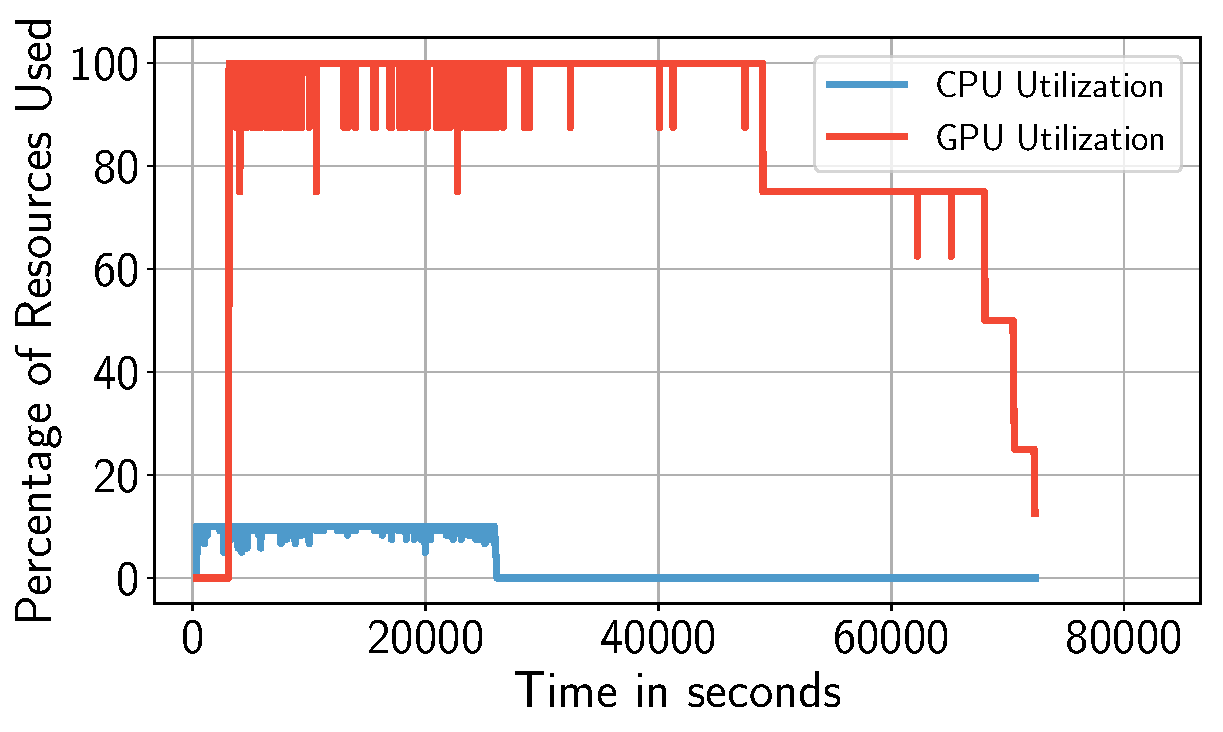
\includegraphics[width=\textwidth]{figures/designs/Design1Utilization.pdf}
        \caption{}
        \label{fig:design1util}
    \end{subfigure}\\
    ~ 
    \begin{subfigure}[b]{0.65\textwidth}
        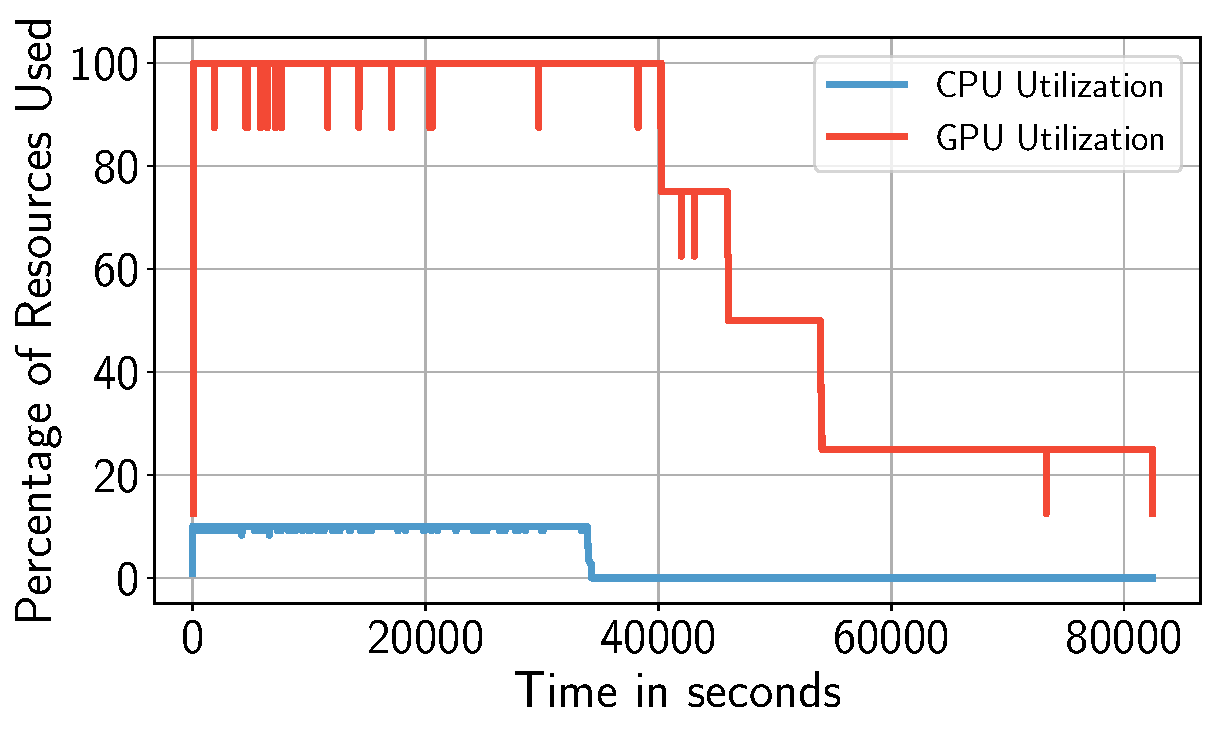
\includegraphics[width=\textwidth]{figures/designs/Design2Utilization.pdf}
        \caption{}
        \label{fig:design2util}
    \end{subfigure}\\
    ~ 
    \begin{subfigure}[b]{0.65\textwidth}
        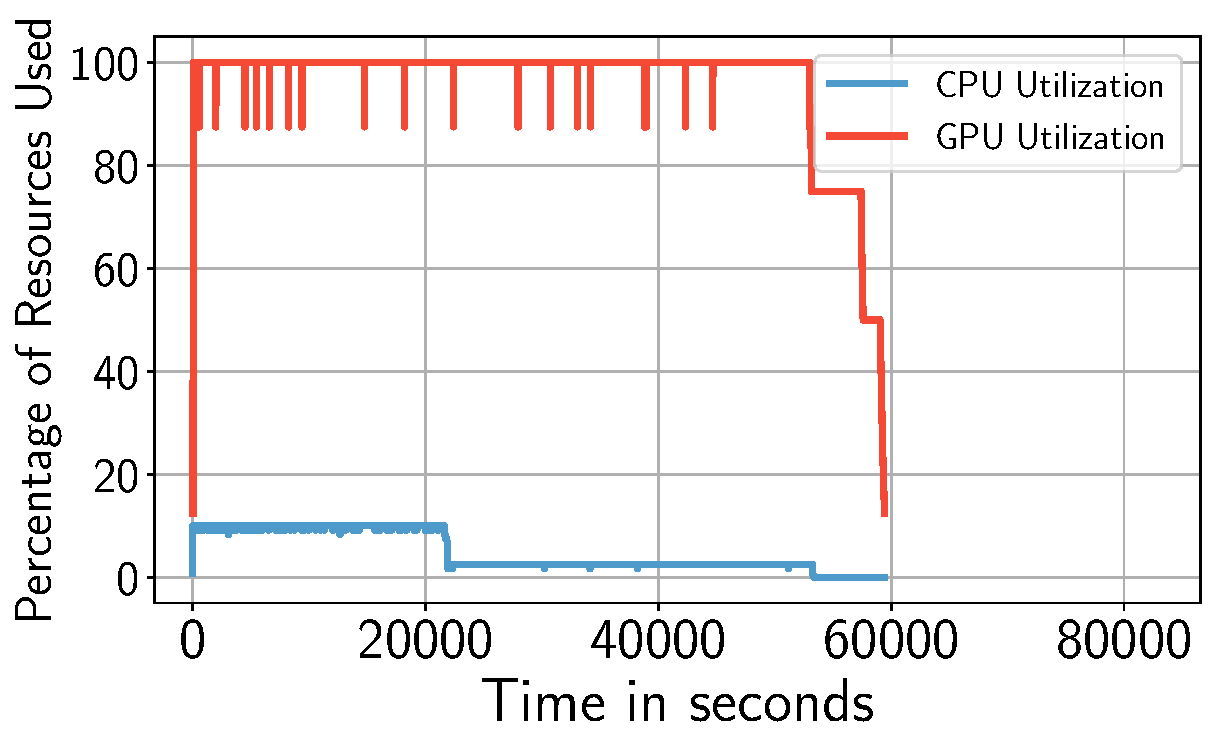
\includegraphics[width=\textwidth]{figures/designs/Design2AUtilization.pdf}
        \caption{}
        \label{fig:design2autil}
    \end{subfigure}
    \caption{Percentage of CPU and GPU utilization for: (a) Design~1; (b) Design~2, and (3) Design~2.A.}
    \label{fig:Utilization}
\end{figure}


Fig.~\ref{fig:design2util} shows resource utilization for a specific run of Design~2.
GPUs are utilized almost immediately as images are becoming available in the queues between $T_{1}$ and $T_{2}$, and this quickly leads to fully utilized resources.
CPUs are utilized for more time compared to Design~1, which is expected due to the longer execution times measured and explained in Experiment~1.
In addition, two GPUs ($25\%$ GPU utilization) are used for more than $20k$ seconds compared to other GPUs.
This shows that the additional execution time of that node was only due to the data size and not due to idle resource time.

Fig.~\ref{fig:design2autil} shows the resource utilization for a specific run of Design~2.A.
For 3 compute nodes out of 4, CPU utilization is shorter than for Design~1 and 2.
For the 4th compute node, CPU utilization is much longer as already explained when discussing $T_{1}$ execution time for Node 3 in Fig.~\ref{fig:design_balancing}, Experiment~1.
As already mentioned, the anomalous behavior of Node 3 supports our hypothesis that compute node performance fluctuations can be much wider than expected.

Fig.~\ref{fig:design2autil} shows that in Design~2.A GPUs are released faster compared to Design~1 and Design~2, leading to a GPU utilization above $90\%$.
As explained in Experiment~1, this is due to differences in data balancing among designs.
This shows the efficacy of two design choices for the concurrent execution of data-driven, compute-intense and heterogeneous workflows: early binding of data to node with balanced distribution of image size alongside the use of local filesystems for data sharing among tasks.

Note that drops in resource utilization are observed in all three designs.
In Design~1, although both CPUs and GPUs were used, in some cases CPU utilization dropped to 6 cores.
Our analysis showed that this happened when RADICAL-Pilot scheduled both CPU and GPU tasks, pointing to an inefficiency in the scheduler implementation.
Design~2 and 2.A CPU utilization drops mostly by one CPU where multiple tiling tasks try to pull from the queue at the same time.
This confirms our conclusions in Experiment~1 about resource competition between middleware and executing tasks.
In all designs, there is no significant fluctuations in GPU utilization, although there are more often in Design~1 when CPU and GPUs are used concurrently.

% ---------------------------------------------------------------------------
\subsection{Experiment~3: Designs Implementation Overheads}\label{ssec:exp3}. 

This experiment studies how the total execution time of our use case workflow varies across Design~1, 2 and 2.A. Fig.~\ref{fig:ttx} shows that Design~1 and 2 have similar total time to execution within error bars, while Design~2.A improves on Design~2 and both are substantially faster than Design~1.
The discussion of Experiment~1 and 2 results explains how these differences relate to the differences in the execution time of $T_{1}$ and $T_{2}$ tasks, and execution concurrency respectively.

\begin{figure}[H]
    \centering
    \begin{subfigure}{0.75\textwidth}
        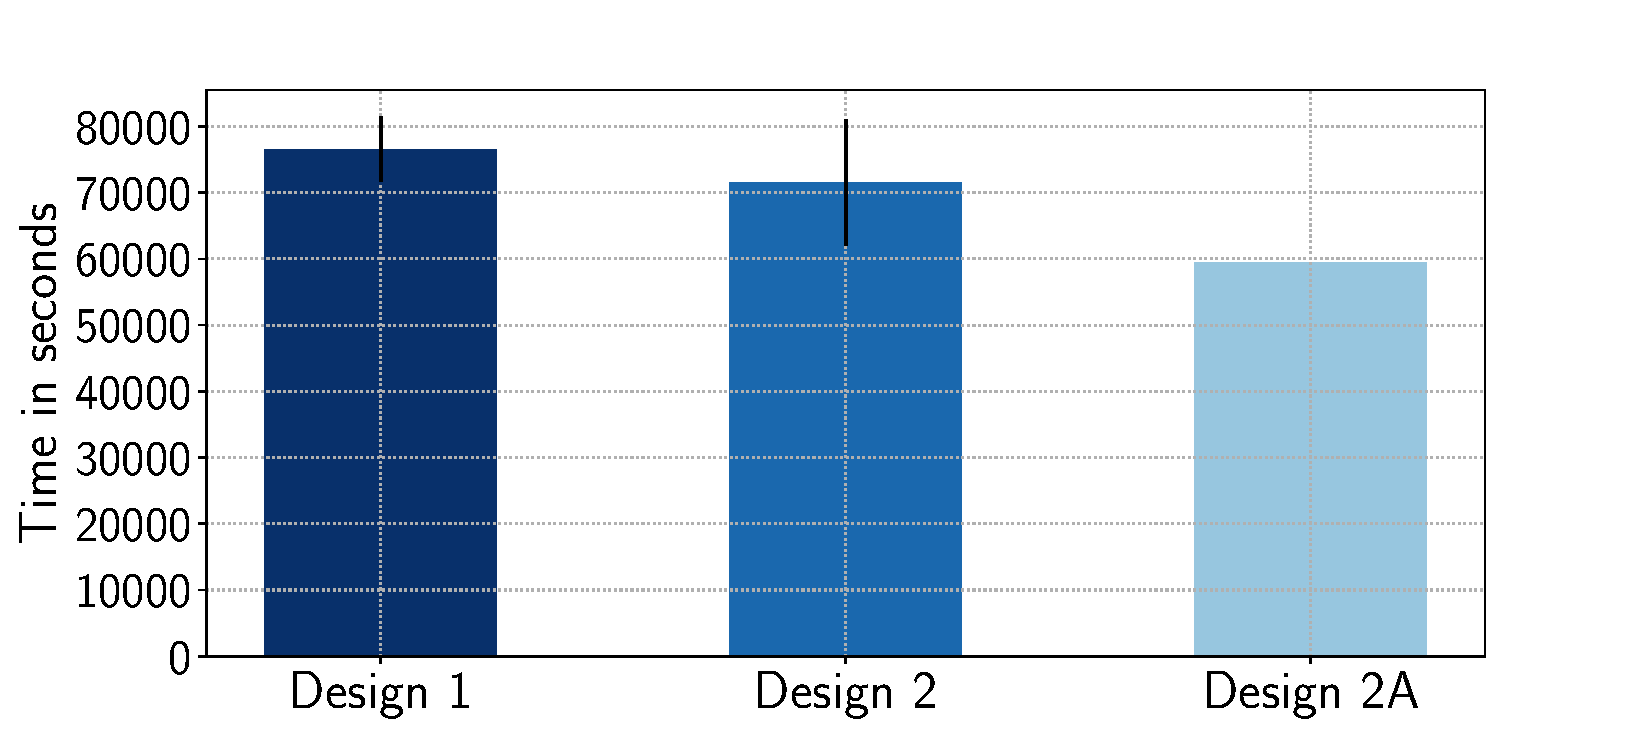
\includegraphics[width=\textwidth]{figures/designs/ttx.pdf}
        \caption{}
        \label{fig:ttx}
    \end{subfigure}\\
    ~
    \begin{subfigure}{0.75\textwidth}
        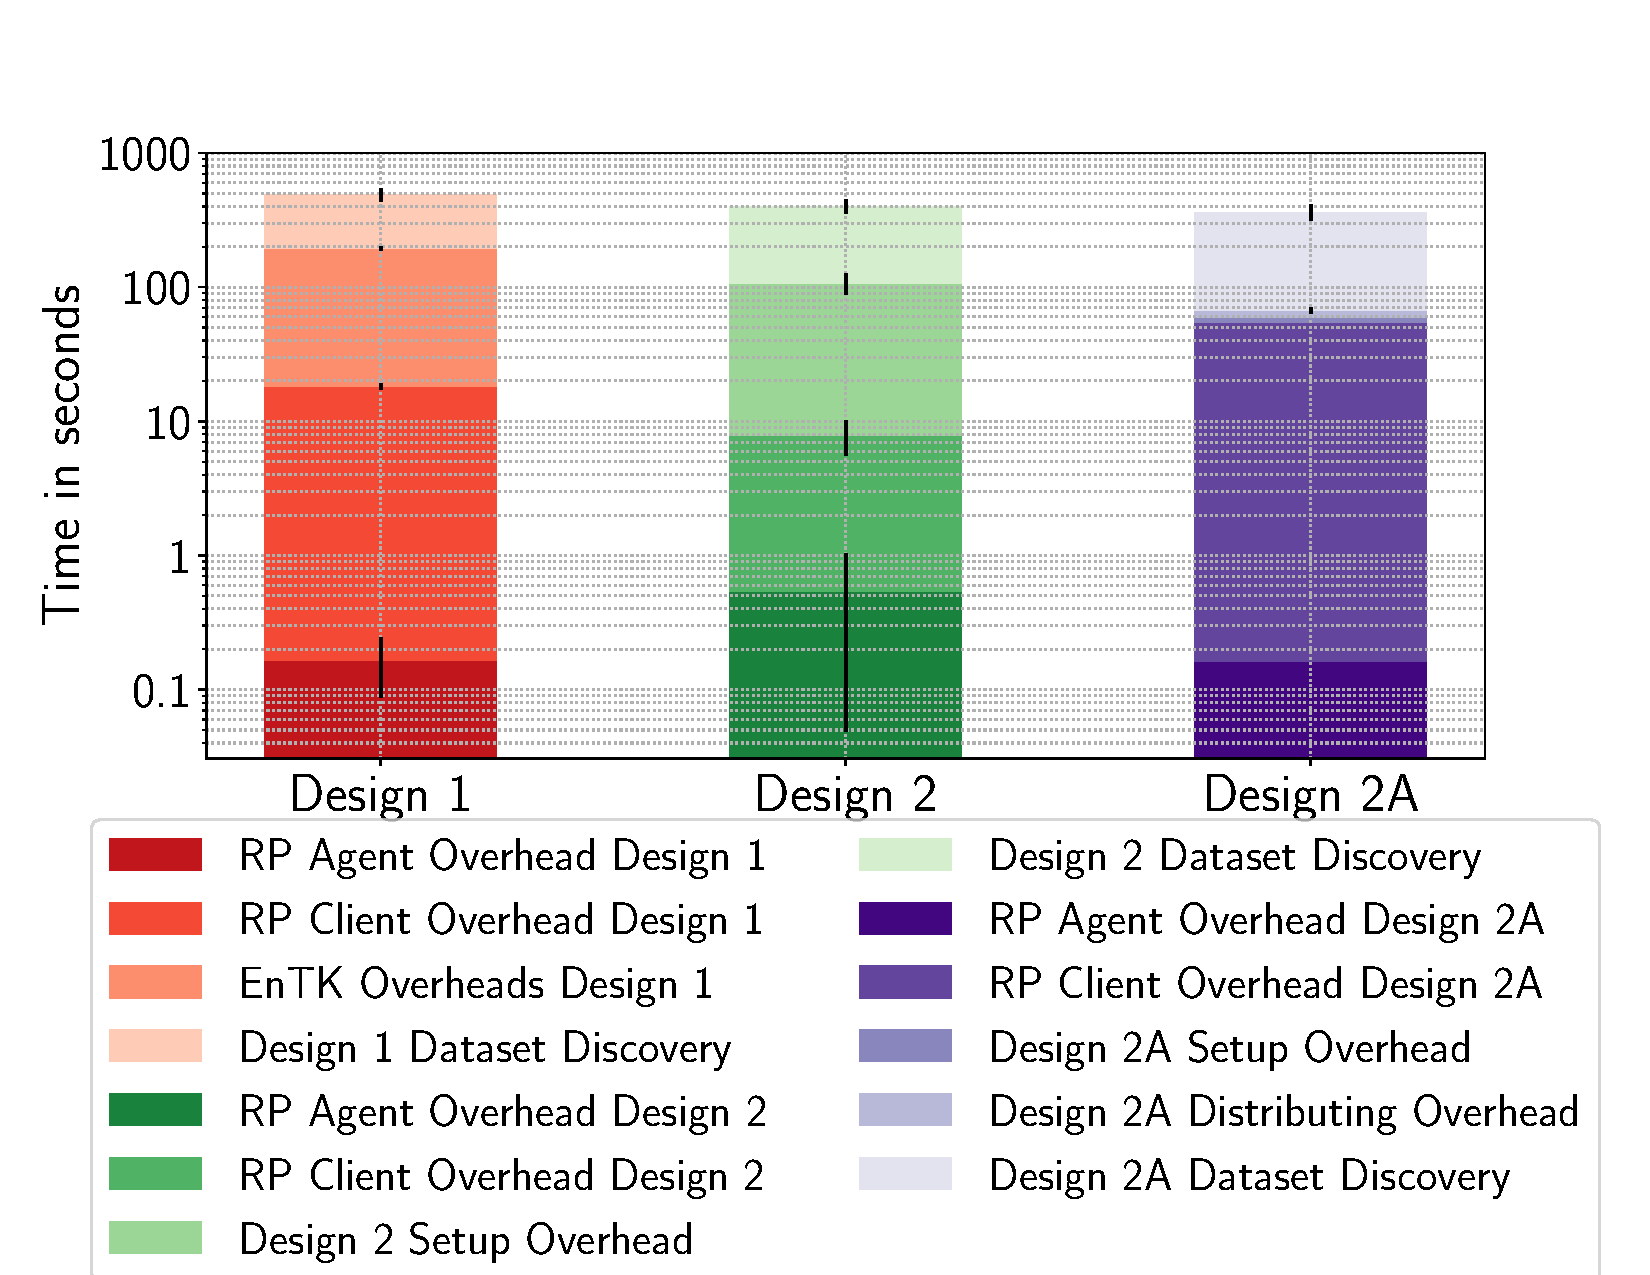
\includegraphics[width=\textwidth]{figures/designs/overheads.pdf}
        \caption{}
        \label{fig:overheads}
    \end{subfigure}
    \caption{(a) Total execution time of Design~1, 2 and 2.A. Design~1 and 2 have similar performance, Design~2.A is the fastest.
        (b) Overheads of Design~1, 2 and 2.A are at least two orders of magnitude less than the total execution time.}\label{fig:overall_performance}
\end{figure}


Fig.~\ref{fig:overheads} shows the overheads of each design implementation.
All three designs overheads are at least two orders of magnitude smaller than the total time to execution.
A common overhead between all designs is the ``Dataset Discovery Overhead''.
This overhead is the time needed to list the dataset and it is proportional to the size of the dataset. 
RADICAL-Pilot has two main components: Agent and Client.
RADICAL-Pilot Agent's overhead is less than a second in all designs while RADICAL-Pilot Client's overhead is in the order of seconds for all three designs.
The latter overhead is proportional to the number of tasks submitted simultaneously to RADICAL-Pilot Agent.

EnTK's overhead in Design~1 includes the time to: (1) create the workflow consisting of $3.1k$ independent pipelines; (2) start EnTK's components; and (3) submit the tasks that are ready to be executed to RADICAL-Pilot. 
This overhead is proportional to the number of tasks in the first stage of a pipeline, and the number of pipelines in the workflow.
EnTK does not currently support partial workflow submission, which would allow us to submit the minimum number of tasks to fully utilize the resources before submitting the rest.
Experiments should be performed to measure the offset between resource utilization optimization and increased time spent in communicating between EnTK and RADICAL-Pilot.

Fig.~\ref{fig:overheads} shows that the dominant overheads of Design~2 is ``Design~2 Setup Overhead''.
This overhead includes setting up and starting queues in each compute node, and starting and shutting down both $T_{1}$ and $T_{2}$ tasks on each node.
Setting up and starting the queues accounts for most of the overhead as we use a conservative waiting time to assure that all the queues are up and ready.
%This can be optimized further reducing the impact of this overhead.

Alongside the overheads already discussed, Design~2.A also introduces an overhead called ``Design~2.A Distributing Overhead'' when partitioning and distributing the dataset over separate nodes.
The average time of this overhead is $7.5$ seconds, with a standard deviation of $3.71$ and is proportional to the dataset and the number of available compute nodes.

In general, Design~2.A shows the best and more stable performance, in terms of overheads, resource utilization, load balancing and total time to execution.
Although Design~2 has similar overheads, even assuming minimization of Setup Overhead, it does not guarantee load balancing as done instead by 2.A.
Design 1 separates the execution in independent pipelines that are independently executed by the runtime system on any available resource.
Based on the results of our analysis, both EnTK and RADICAL-Pilot can be configured to implement early binding of images to each compute node as done in Design~2.A.
Nonetheless, Design~1 would still require executing a task for each image, imposing bootstrap and tear down overheads for each task.

\section{Discussion and Conclusions}
\label{sec:des_concl}

While designs 1, 2 and 2.A successfully support the execution of the paradigmatic workflow described in~\S\ref{sec:ucase}, our experiments show that for the metrics considered, Design~2.A is the one offering the better overall performance.
Generalizing this result, use cases that are both data-driven and compute-intense benefit from early binding of data to compute node so to maximize data and compute affinity and equally balance input across nodes.
This approach minimizes the overall time to completion of this type of workflows while maximizing resource utilization.

Our analysis also shows the limits of an approach where pipelines, i.e., compute tasks, are late bound to compute nodes.
In program-based designs, the overhead of bootstrapping programs needs to be minimized insuring that each pipeline processes as much input as possible (e.g. images).
In presence of large amount of data, late binding implies copying, replicating or accessing data over network and at runtime.
We showed that, in contemporary HPC infrastructures, this is too costly both for resource utilization and total time to completion.

When executing workflows as part of a computational campaign, it is important to efficiently utilize available resources.
Our design evaluation provides us with information on how to implement the workflows of a campaign effectively.
In addition, our overheads characterization provides us with a baseline to evaluate the production grade workflow implementations.


%Infrastructure-wise, our experiments show the limits imposed by an unbalance between number of CPU cores and available memory.
%Given data-driven computation where multi GB images need processing, we were able to use just $10\%$ of the available cores due to the amount of RAM required.
%This applies also to the unbalance between CPUs and GPUs: use cases with heterogeneous tasks would benefit from a n higher GPU/CPU ratio.



%These results apply to the evaluation of the design of existing and future computing frameworks. 
%For example, we are extending both EnTK and RADICAL-Pilot to implement Design~2.A.
%We will use our overheads characterization as a baseline to evaluate our production-grade implementation and further improve the efficiency of our middleware. 
%Further, we will apply the presented experimental methodology to other use cases and infrastructures, measuring the trade offs imposed by other types of task heterogeneity, including multi-core or multi-GPU tasks that extends beyond a single compute node.


%%%%%%%%%%%%%%%%%%%%%%%%%%%%%%%%%%%%%%%%%%%%%%%%%%%%%%%%%%%%%%%%%%%%%%%%%%%%%%%%
%For our CNN architecture, we use a U-Net~\cite{ronneberger2015u} variant that counts seals with an added regression branch and locates them using a seal intensity heat map.
%To train our CNN, we use a training set of 53 WV03 images, with $88k$ hand-labeled tiles, where every tile has a correspondent seal count and a class label (i.e., seal vs. non-seal).
%For hyper-parameter search, we train CNN variants for 75 epochs (i.e., 75 complete runs through the training set) using an Adam optimizer~\cite{kingma2014adam} with a learning rate of $10^{-3}$ and tested against a validation set.
%The validation set consists of $10\%$ of the training set.
%In addition, we randomized the WV03 image selection so that a validation tile does not overlap with a training one.
%Testing was performed on 5 WV03 images.
%Double observer seal counting was performed and model detection results were compared to observer consensus detections.
%Furthermore, we avoid double counting by setting a minimum distance boundary between neighboring seals and keeping those where the model was more confident.
